\providecommand\ExamFontPath{../../../字体/}
\documentclass[fontset=exam]{exam-zh}
\usepackage{longtable,booktabs,array,calc,multirow,fvextra}
\usepackage[normalem]{ulem}
\providecommand{\hl}[1]{#1}
\providecommand{\ul}[1]{\uline{#1}}
\DefineVerbatimEnvironment{verbatim}{Verbatim}{breaklines=true,fontsize=\small}
\providecommand{\tightlist}{\setlength{\itemsep}{0pt}\setlength{\parskip}{0pt}}
\newcommand{\pandocbounded}[1]{#1}
\setlength{\emergencystretch}{3em}
\setlength{\tabcolsep}{2pt}
\examsetup{page/size=a4paper}
\title{厦门大学期末考试 A 卷}
\subject[9em]{大学物理 B（下）}
\begin{document}
\maketitle
\fancyfoot[C]{第 \thepage 页（共 \pageref*{LastPage} 页）}
\noindent\makebox[\linewidth][c]{考试时间：2025 年 01 月}\par
\pdfbookmark[1]{一、选择题：本题共10小题，每小题2分，共20分。请把正确答案填写在答题纸的正确位置。每小题给出的四个选项中只有一个选项}{section3}

\par\medskip{\heiti

一、选择题：本题共 10 小题，每小题 2 分，共 20 分。请把正确答案填写在答题纸的正确位置。每小题给出的四个选项中只有一个选项正确。错选、多选或未选的得 0 分。

\par}\smallskip

1． 白光通过玻璃三棱镜会发生色散现象。这说明不同频率的光在玻璃中传播速度不同。根据折射率与光速的关系可知（ ）光在玻璃中传播速度最慢。

（A）红 （B）绿 （C）黄 （D）紫

2． 平面镜成像的横向放大率为（ ）

（A）1 （B）-1 （C）∞ （D）0

3． 光在真空中和介质中传播时，正确的描述是（ ）

（A）波长不变，介质中的波速减小 （B）介质中的波长变短，波速不变

（C）频率不变，介质中的波速减小 （D）介质中的频率减小，波速不变

4．双缝干涉实验装置如图所示，若双缝所在的平板稍微向上平移，其他条件不变，则屏上的干涉条纹（ ）

（A）向下平移，且条纹间距不变

（B）向上平移，且条纹间距不变

（C）不移动，但条纹间距改变

（D）向上平移，且间距改变

5． 两块平玻璃构成空气劈形膜，左边为棱边，用单色平行光垂直入射。若上面的平玻璃以棱边为轴，沿逆时针方向作微小转动，则干涉条纹的（ ）

（A）间隔变小，并向棱边方向平移

（B）间隔变大，并向远离棱边方向平移

（C）间隔不变，向棱边方向平移

（D）间隔变小，并向远离棱边方向平移

6． 在夫琅和费衍射实验中，用单色光平行垂直入射后，在光屏上产生衍射条纹，对于屏上的第二级明纹中心，相应的单缝所分成的半波带数目为（ ）

（A）2 （B）3 （C）4 （D）5

7． 对一个作简谐振动的物体，下列哪种说法是正确的？（ ）

（A）物体处在最大正位移处，速率和加速度大小亦为最大值；

（B）物体位于平衡位置时，速率和加速度亦为 0；

（C）物体位于平衡位置时，速率最大，加速度为 0；

（D）物体处在最大负位移处，速率最大，加速度为 0。

8． 竖直悬挂的轻质弹簧下端固定一小球构成一弹簧振子，其简谐振动周期为\emph{T}。将小球浸没在水中，让弹簧振子作竖直方向振动。在振动过程中，小球受到的浮力保持不变，且不计其他阻力，则（ ）

（A）振子仍作简谐振动，但周期小于\emph{T}；

（B）振子仍作简谐振动，但周期大于\emph{T}；

（C）振子仍作简谐振动，但周期等于\emph{T}；

（D）振子不作简谐振动。

9． 在简谐波传播过程中，沿波传播方向相距半波长的两点的振动速度必定（ ）

（A）大小相同，方向相反； （B）大小和方向均相同；

（C）大小不同，方向相同； （D）大小不同而方向相反。

10．一列简谐机械波，在某一时刻，媒质中质元刚好经过平衡位置，关于该质元能量描述正确的是（ ）

（A）动能最大，势能也最大； （B）动能最小，势能也最小；

（C）动能最大，势能最小； （D）动能最小，势能最大。

\pdfbookmark[1]{二、填空题：本大题共10空，每空2分，共20分。请把正确答案填写在答题纸的正确位置。错填、不填均无分。}{section39}

\par\medskip{\heiti

二、填空题：本大题共 10 空，每空 2 分，共 20 分。请把正确答案填写在答题纸的正确位置。错填、不填均无分。

\par}\smallskip

1．一种玻璃对红光（\emph{λ}=633nm）的折射率为 1.52。这种玻璃在空气中对此红光发生全反射的临界角为\underline{\hspace{1.5cm}}。

2．用一折射率为 1.5 的玻璃制成的薄凸透镜置于空气中，前后两球面的曲率半径均为 40cm，则此透镜的焦距为\underline{\hspace{1.5cm}}cm。

3．平行单色光垂直入射在缝宽为\emph{a}=0.15mm 的单缝上。缝后有焦距为\emph{f}=400mm 的凸透镜，在其焦平面上放置观察屏幕。现测得屏幕上中央明条纹两侧的两个第三级暗纹之间的距离为 8mm，则入射光的波长为\underline{\hspace{2cm}}nm。

4．用波长为\emph{λ}的单色平行光垂直照射到一个光栅上，该光栅的光栅常数\emph{d}=2μm，在光栅后方放置一个焦距\emph{f} =0.500 m 的凸透镜，光通过透镜后汇聚在焦平面的屏幕上。测得屏幕上第一级主极大明纹与中央明纹的距离\emph{l}=0.1667m．则入射光波长\emph{λ}=\underline{\hspace{2cm}}nm．

\par\medskip{\centering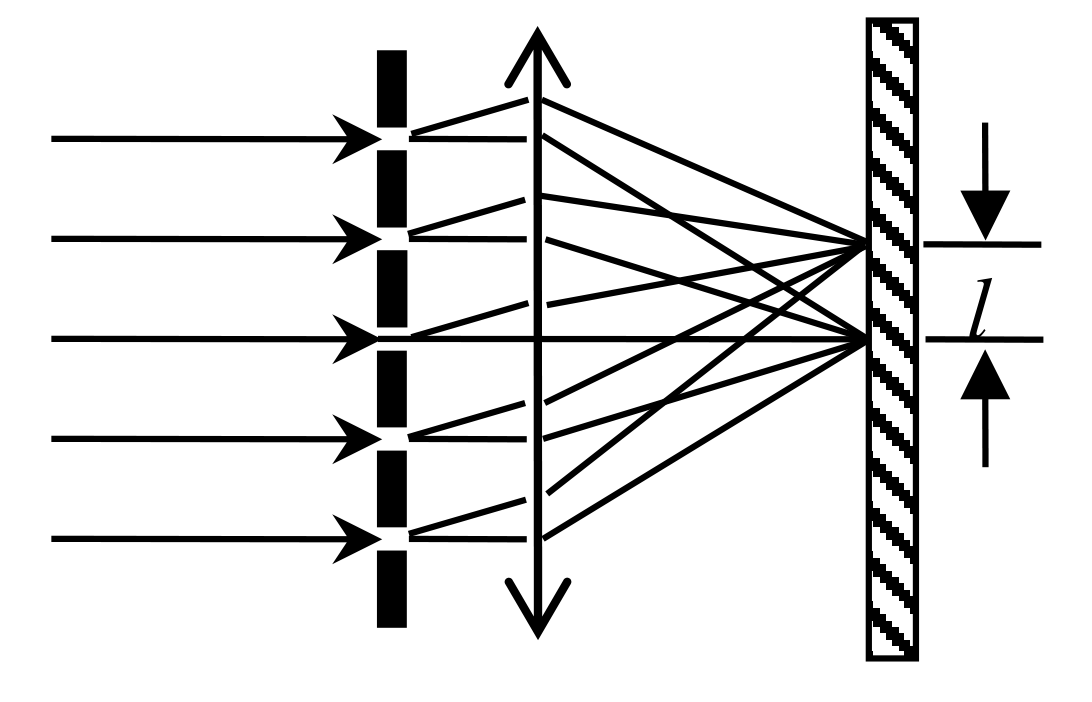
\includegraphics[width=5cm,height=4cm,keepaspectratio]{figures/grating4.png}\par}\medskip

5．一束自然光从空气投射到玻璃表面上(空气折射率为 1)，当折射角为 30°时，反射光是完全线偏振光，则此玻璃板的折射率等于\underline{\hspace{2cm}}。

6． 光强为\emph{I}\textsubscript{0}的自然光垂直通过两个偏振片后，出射光强\emph{I=I}\textsubscript{0}/8，则两个偏振片的偏振化方向之间的夹角为\underline{\hspace{2cm}}。

7． 用 40N 的力拉一根轻弹簧，可使其伸长 20cm，此弹簧下应挂 kg 的物体，才能使弹簧振子做简谐振动的周期 T=0.2π s。

8． 一个物体同时参与同一直线上的两个简谐振动：

\(x_{1} = 0.03cos(4\pi t + \frac{\pi}{3})\) （SI）

\(x_{2} = 0.05cos(4\pi t - \frac{2\pi}{3})\) （SI）

合成振动的振动方程为\emph{x}=\underline{\hspace{1.5cm}}（SI）。

9．已知一平面简谐波频率为 1000Hz，波速为 300m/s，则波上相位差为\emph{π}/4 的两点之间的距离为\underline{\hspace{1.5cm}}m。

10． 两相干波源\emph{S}\textsubscript{1}、\emph{S}\textsubscript{2}之间的距离为 20m，两波的波速为\emph{u}=400m/s，频率\emph{v}=100Hz，振幅\emph{A}相等且\emph{A}=0.02m，并且已知\emph{S}\textsubscript{1}的相位比\emph{S}\textsubscript{2}的相位超前\emph{π}，则\emph{S}\textsubscript{1}与\emph{S}\textsubscript{2}连线中点的振幅为\underline{\hspace{1.5cm}}m。

\pdfbookmark[1]{三、计算题：本题12分。请在答题纸上按题序作答，并标明题号。}{section54}

\par\medskip{\heiti

三、计算题：本题 12 分。请在答题纸上按题序作答，并标明题号。

\par}\smallskip

一支蜡烛位于一凹面镜前 0.5m 处，其像位于距镜顶 1m 远处的屏上，求：

（1）凹面镜的半径和焦距；

（2）如果蜡烛火焰的高度为 5mm，则屏上火焰的像高为多少？

\pdfbookmark[1]{四、计算题：本题12分。请在答题纸上按题序作答，并标明题号。}{section58}

\par\medskip{\heiti

四、计算题：本题 12 分。请在答题纸上按题序作答，并标明题号。

\par}\smallskip

如图，波长为 6800Å的平行光垂直照射到\emph{L}＝0.12m 长的两块玻璃片上，两玻璃片一边相互接触，另一边被直径\emph{d}=0.048mm 的细钢丝隔开．求：

(1)两玻璃片间的夹角；

(2)相邻两明条纹间空气膜的厚度差；

(3)相邻两暗条纹的间距；

(4) 在这 0.12 m 内，反射光干涉条纹中明纹数目。（不考虑钢丝遮挡光线）

\par\medskip{\centering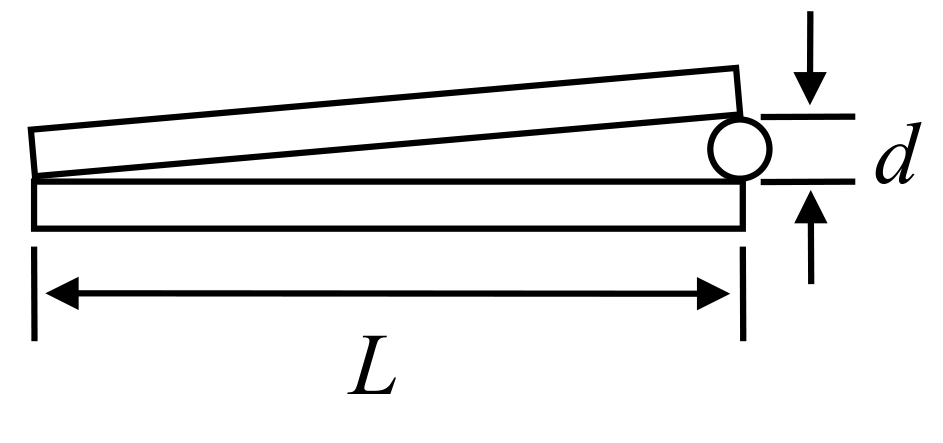
\includegraphics[width=5cm,height=4cm,keepaspectratio]{figures/glass4.png}\par}\medskip

\pdfbookmark[1]{五、计算题：本题12分。请在答题纸上按题序作答，并标明题号。}{section66}

\par\medskip{\heiti

五、计算题：本题 12 分。请在答题纸上按题序作答，并标明题号。

\par}\smallskip

一光栅的光栅常数为 0.1mm，缝宽为 0.02mm，用波长为 4800Å的平行单色光垂直入射光栅，光栅后放一焦距为 50cm 的透镜。试求：

（1）透镜焦平面上单缝衍射中央明条纹的宽度；

（2）单缝衍射的中央明条纹包迹内有多少条光栅衍射主极大明条纹?

\pdfbookmark[1]{六、计算题：本题12分。请在答题纸上按题序作答，并标明题号。}{section70}

\par\medskip{\heiti

六、计算题：本题 12 分。请在答题纸上按题序作答，并标明题号。

\par}\smallskip

一质量为 10×10\textsuperscript{-3}kg 的物体沿\emph{x}轴方向作谐振动，取平衡位置处为坐标原点，振幅为 24cm，周期为 4.0s，当\emph{t}=0 时位移为+24cm．求：

（1）\emph{t}=0.5s 时，物体所在的位置及此时所受力的大小和方向；

（2）由起始位置运动到\emph{x}=12cm 处所需的最短时间；

（3）在\emph{x}=12cm 处物体的机械能。

\pdfbookmark[1]{七、计算题：本题12分。请在答题纸上按题序作答，并标明题号。}{section75}

\par\medskip{\heiti

七、计算题：本题 12 分。请在答题纸上按题序作答，并标明题号。

\par}\smallskip

设入射波的方程\(y_{1} = Acos\left\lbrack {2\pi\left( {\frac{x}{\lambda} + \frac{t}{T}} \right)} \right\rbrack\)在\emph{x}=0 处发生反射，反射点为一固定端，设反射时无能量损失，求：

（1）反射波的方程式；

（2）合成的驻波方程式；

（3）波腹和波节的位置。

\end{document}
